\subsection{Năng lượng}
\begin{frame}
    \frametitle{Các bài toán quen thuộc}
    \begin{columns}
        \begin{column}{0.5\textwidth}
            \vspace{-14pt}

            \begin{figure}
                \centering
                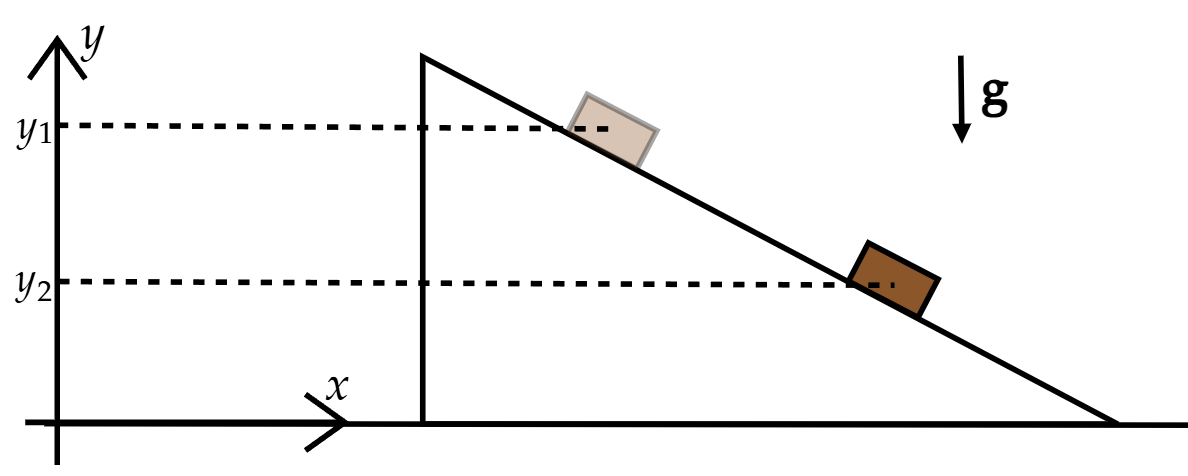
\includegraphics[width=7cm, height=3cm]{Content/Figure/gravity_energy.png}
            \end{figure}
            \[\frac{d}{dt}\left(\frac{mv^2}{2}-mgy\right)=0.\]
            \[\Delta\left(\frac{mv^2}{2}\right)-\int_{y_1}^{y_2}(-mg)dy=0.\]
        \end{column}
        \begin{column}{0.5\textwidth}
            \vspace{-14pt}

            \begin{figure}
                \centering
                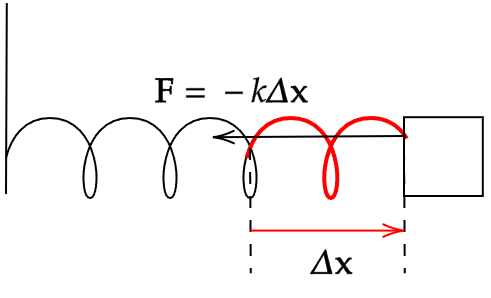
\includegraphics[width=5cm, height=3cm]{Content/Figure/springmass.png}
            \end{figure}
            \[\frac{d}{dt}\left(\frac{mv^2}{2}+\frac{k(\Delta x)^2}{2}\right)=0.\]
             \[\Delta\left(\frac{mv^2}{2}\right)-\int_{ x_1}^{x_2}(-k\Delta x)dx =0.\]
        \end{column}
    \end{columns}
\end{frame}
\begin{frame}
    \frametitle{Động năng, công, và thế năng}
    \begin{itemize}
        \item Đại lượng \(K=\frac{mv^2}{2}\) được gọi là động năng.
        \item Đại lượng \(A=\int_{q_1}^{q_2}F_q dq\) được gọi là công.
        \item Đại lượng \(V(q)=-\int_{\mathcal{O}}^{q}F_q(q)dq\) được gọi là thế năng.
    \end{itemize}
    Định lý biến thiên động năng: \[\frac{dK}{dt}=\sum \mathbf{F}\cdot\mathbf{v}.\]
    Nếu công của tất cả các lực tác dụng có thể được viết dưới dạng một hàm thế năng \(V(q)\), thì \emph{cơ năng} bảo toàn:
    \[E=K+V=const.\]
    \vspace{-16pt}

    Chú ý: Không phải công của mọi lực chỉ phụ thuộc vào toạ độ đều có thể viết dưới dạng thế năng.
\end{frame}
\begin{frame}
\frametitle{Năng lượng của hệ}
\[E=\sum_{i}\frac{m_i v_{i}^2}{2}+V.\]
\[V=V_{12}+V_{13}+\cdots +V_{V1N}+V_{23}+\cdots +V_{(N-1)N}=\sum_{i<j} V_{ij}.\]
Ta không biết được thế năng của các tương tác vi mô, do đó trong phần lớn trường hợp, phần năng lượng này không được tính vào sự bảo toàn cơ năng. Sự chuyển hoá năng lượng với các nguyên nhân không rõ ràng được gọi là tỏa nhiệt.
\vspace{8pt}

Sự bảo toàn năng lượng có phụ thuộc vào cách chọn hệ.
\end{frame}